\subsection{Versterking}\label{sec:versterking}
Tussen de uitgang van de pH sensor en het filter zit in het signaalverwerking blokschema in \cref{fig:analogeBewerkingsFunctie} een versterker.

\begin{figure}[!htbp]
    \centering
    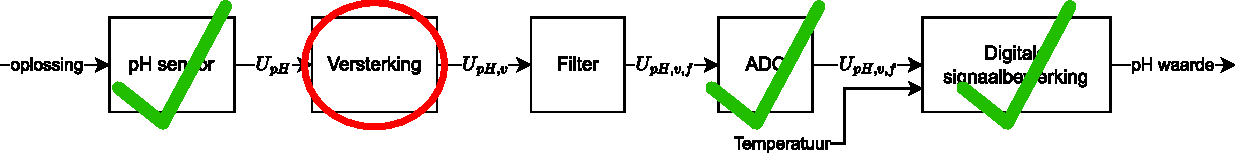
\includegraphics[width=0.95\textwidth]{signaalverwerking_versterker}
    \caption{Het onderdeel van \cref{fig:analogeBewerkingsFunctie} waar de spanningsreferentie zich in bevindt.}
    \label{fig:versterkerInSchema}
\end{figure}

Op dit moment lijkt het erg plausibel om de pH waarde uit te lezen zonder een versterker te gebruiken. Een versterker voegt toe aan het energieverbruik van het systeem. Dit is waarom er is besloten om nog geen versterker toe te voegen aan het systeem, zodat later gekeken kan worden of dit resulteert in een werkende sensormodule.